\documentclass{beamer}
\usepackage[utf8]{inputenc}

\usetheme{Madrid}
\usecolortheme{default}
\usepackage{amsmath,amssymb,amsfonts,amsthm}
\usepackage{txfonts}
\usepackage{tkz-euclide}
\usepackage{listings}
\usepackage{adjustbox}
\usepackage{array}
\usepackage{tabularx}
\usepackage{gvv}
\usepackage{lmodern}
\usepackage{circuitikz}
\usepackage{tikz}
\usepackage{graphicx}

\setbeamertemplate{page number in head/foot}[totalframenumber]

\usepackage{tcolorbox}
\tcbuselibrary{minted,breakable,xparse,skins}



\definecolor{bg}{gray}{0.95}
\DeclareTCBListing{mintedbox}{O{}m!O{}}{%
  breakable=true,
  listing engine=minted,
  listing only,
  minted language=#2,
  minted style=default,
  minted options={%
    linenos,
    gobble=0,
    breaklines=true,
    breakafter=,,
    fontsize=\small,
    numbersep=8pt,
    #1},
  boxsep=0pt,
  left skip=0pt,
  right skip=0pt,
  left=25pt,
  right=0pt,
  top=3pt,
  bottom=3pt,
  arc=5pt,
  leftrule=0pt,
  rightrule=0pt,
  bottomrule=2pt,
  toprule=2pt,
  colback=bg,
  colframe=orange!70,
  enhanced,
  overlay={%
    \begin{tcbclipinterior}
    \fill[orange!20!white] (frame.south west) rectangle ([xshift=20pt]frame.north west);
    \end{tcbclipinterior}},
  #3,
}
\lstset{
    language=C,
    basicstyle=\ttfamily\small,
    keywordstyle=\color{blue},
    stringstyle=\color{orange},
    commentstyle=\color{green!60!black},
    numbers=left,
    numberstyle=\tiny\color{gray},
    breaklines=true,
    showstringspaces=false,
}
%------------------------------------------------------------
%This block of code defines the information to appear in the
%Title page
\title %optional
{1.7.12}
\date{August 27,2025}
%\subtitle{A short story}

\author % (optional)
{Rathlavath Jeevan-AI25BTECH11026}



\begin{document}


\frame{\titlepage}
\begin{frame}{Question}
\textbf{} Find the value of $k$, if the points $P(5,4)$, $Q(7,k)$ and $R(9,-2)$ are collinear. 

\textit{Hint:} Three points $P(x_1,y_1)$, $Q(x_2,y_2)$, $R(x_3,y_3)$ are collinear if the area of the triangle formed by them is zero.\\
\\
\end{frame}


\begin{frame}{Theoretical Solution}
\textbf{Solution:} \\
\begin{align}
\vec P=\myvec{5\\4},\qquad
\vec Q=\myvec{7\\k},\qquad
\vec R=\myvec{9\\-2}
\end{align}

 \textbf{Collinearity via rank}
Three points \(P,Q,R\) are collinear iff
\begin{align}
\operatorname{rank}\!\myvec{\; \vec Q-\vec P \;\; \vec R-\vec P \;}=1.
\end{align}
Compute the direction columns:
\begin{align}
\vec Q-\vec P=\myvec{7-5\\k-4}=\myvec{2\\k-4},\qquad
\vec R-\vec P=\myvec{9-5\\-2-4}=\myvec{4\\-6}.
\end{align}
Hence the collinearity matrix is
\begin{align}
M=\myvec{\,2 & 4\\ k-4 & -6\,}.
\end{align}

\textbf{Row reduction (rank\,=\,1)}
\end{frame}
\begin{frame}{Theoretical Solution}
\begin{align}
\myvec{\,2 & 4\\k-4 & -6\,}
\;\xrightarrow{\,R_1\leftarrow \tfrac12 R_1\,}\;
\myvec{\,1 & 2\\k-4 & -6\,}
\;\xrightarrow{\,R_2\leftarrow R_2-(k-4)R_1\,}\;
\myvec{\,1 & 2\\0 & 2(1-k)\,}.
\end{align}
For rank\((M)=1\), the second row must be the zero row:
\begin{align}
2(1-k)=0 \;\;\Rightarrow\;\; k=1.
\end{align}

\textbf{Conclusion}
For \(k=\boxed{1}\), the three points \(P(5,4),\,Q(7,k),\,R(9,-2)\) are collinear.


\end{frame}




\begin{frame}[fragile]
    \frametitle{C Code }

    \begin{lstlisting}
#include <stdio.h>

int main() {
    int x1 = 5, y1 = 4;
    int x2 = 7, y2;   // y2 = k
    int x3 = 9, y3 = -2;
    int k;

    // Equation: x1(y2 - y3) + x2(y3 - y1) + x3(y1 - y2) = 0
    // Substituting values
    // 5(k - (-2)) + 7((-2) - 4) + 9(4 - k) = 0
    // Solve manually inside program:

    // Simplified form: -4k + 4 = 0 => k = 1
    k = 1;
      \end{lstlisting}
\end{frame}

    \begin{frame}[fragile]
    \frametitle{C Code }

    \begin{lstlisting}

    printf("The value of k is: %d\n", k);

    return 0;
}

    \end{lstlisting}
\end{frame}





\begin{frame}[fragile]
    \frametitle{Python Code }
    \begin{lstlisting}
    
import matplotlib.pyplot as plt

# Given points
P = (5, 4)
R = (9, -2)

# Find k using collinearity condition
slope_PR = (R[1] - P[1]) / (R[0] - P[0])
k = slope_PR * (7 - 5) + 4
Q = (7, k)

# Plotting the points and line
plt.figure(figsize=(6,6))
plt.plot([P[0], Q[0], R[0]], [P[1], Q[1], R[1]], 'ro')  # points
plt.plot([P[0], Q[0], R[0]], [P[1], Q[1], R[1]], 'b-')  # line
\end{lstlisting}
\end{frame}
\begin{frame}[fragile]
    \frametitle{Python Code }
    \begin{lstlisting}
        
   
# Annotating points
plt.text(P[0]+0.1, P[1], f"P{P}")
plt.text(Q[0]+0.1, Q[1], f"Q{Q}")
plt.text(R[0]+0.1, R[1], f"R{R}")

plt.axhline(0, color='black', linewidth=0.5)
plt.axvline(0, color='black', linewidth=0.5)
plt.grid(True)
plt.title("Collinear Points Diagram")
plt.xlabel("x-axis")
plt.ylabel("y-axis")

# Save as image
plt.savefig("collinear_points.png", dpi=300)
plt.show()
\end{lstlisting}
\end{frame}
\begin{frame}[fragile]
    \frametitle{Python Code }
    \begin{lstlisting}
print("Value of k:", k)
print("Graph saved as 'collinear_points.png'")
 \end{lstlisting}
\end{frame}


\begin{frame}{Plot}
    \centering
    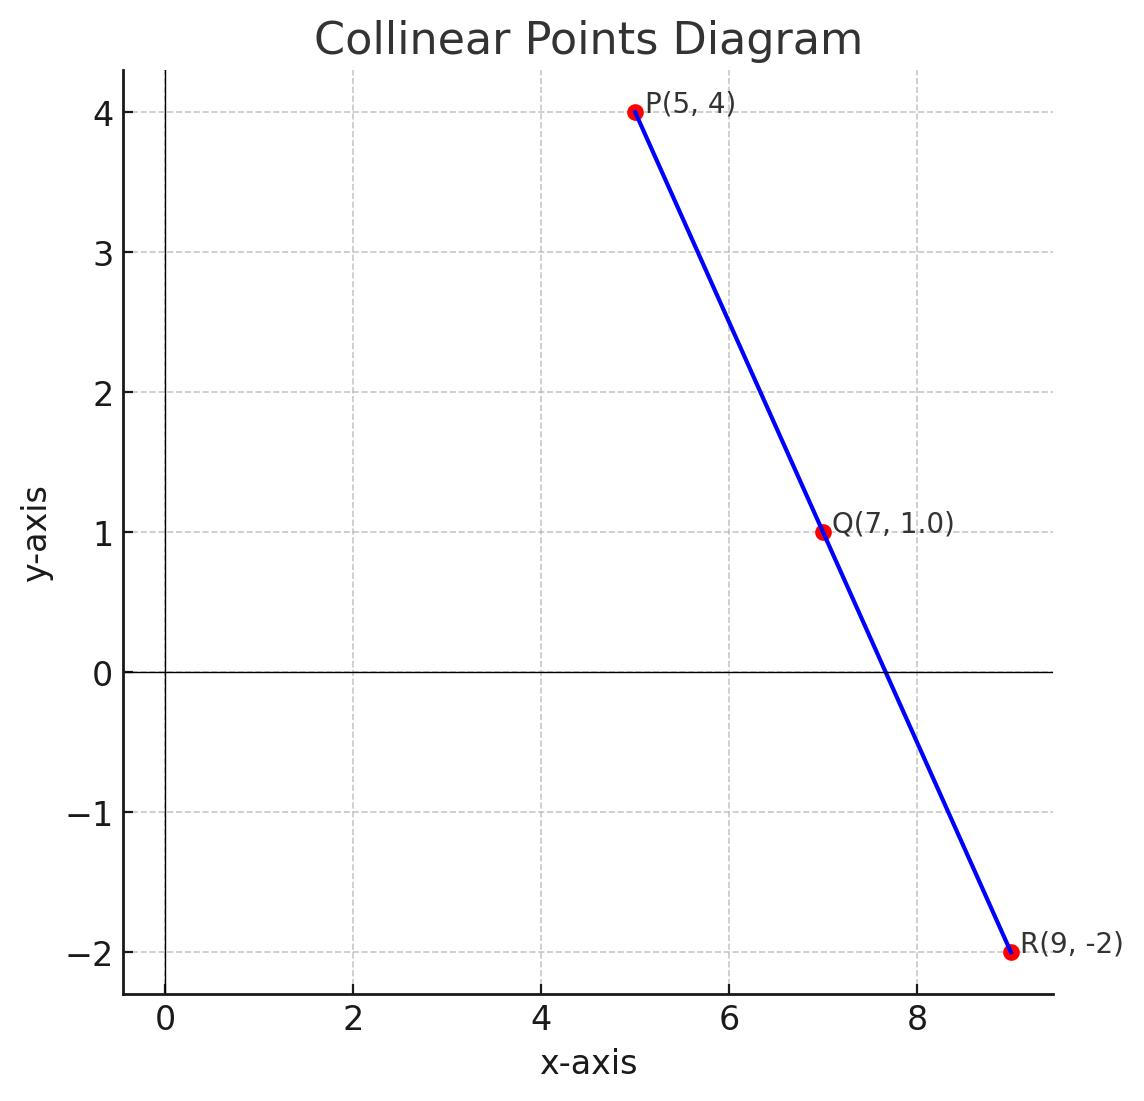
\includegraphics[width=\columnwidth, height=0.8\textheight, keepaspectratio]{beamer/figs/ASSIGN2.jpeg}     
\end{frame}




\end{document}